\documentclass[11pt,a4paper]{article}
\usepackage[margin=22mm,headheight=16pt,footskip=12mm]{geometry}
\usepackage[T1]{fontenc}
\usepackage[utf8]{inputenc}
\usepackage{lmodern,amsmath,amssymb,graphicx,xcolor,booktabs,longtable,array,tabularx}
\usepackage{tikz,float,caption,fancyhdr,titlesec,url,lscape}
\usetikzlibrary{arrows.meta,positioning,calc}
\definecolor{navy}{HTML}{16324F}
\definecolor{teal}{HTML}{007F86}
\definecolor{pale}{HTML}{EAF5F5}
\definecolor{ink}{HTML}{243646}
\definecolor{amber}{HTML}{A45C13}
\pdfinfo{/Title (Inverse-GPR Virtual-Fuel PI Controller) /Author (T-MATS Controller Development Study)}
\urlstyle{tt}
\setlength{\parindent}{0pt}
\setlength{\parskip}{5pt plus 1pt minus 1pt}
\setlength{\emergencystretch}{2em}
\widowpenalty=10000\clubpenalty=10000
\linespread{1.05}
\titleformat{\section}{\Large\sffamily\bfseries\color{navy}}{\thesection}{.7em}{}
\titleformat{\subsection}{\large\sffamily\bfseries\color{teal}}{\thesubsection}{.7em}{}
\titlespacing*{\section}{0pt}{19pt}{8pt}
\titlespacing*{\subsection}{0pt}{13pt}{5pt}
\captionsetup{font=small,labelfont={bf,color=navy},skip=8pt}
\pagestyle{fancy}\fancyhf{}
\fancyhead[L]{\small\sffamily\color{navy}R3 / AMBIENT AND SPEED CYCLE}
\fancyhead[R]{\small\sffamily T-MATS control study}
\fancyfoot[L]{\scriptsize\color{ink}Frozen R3 and base PI / 120 s cycle}
\fancyfoot[R]{\small\thepage}
\renewcommand{\headrulewidth}{.3pt}
\tikzset{block/.style={draw=navy!55,fill=navy!3,rounded corners=3pt,minimum height=.92cm,align=center,font=\sffamily\small,inner sep=5pt},
gp/.style={block,draw=teal,fill=pale},plant/.style={block,draw=navy,fill=navy!12},
sum/.style={circle,draw=navy,minimum size=.68cm,fill=white,font=\large},
arr/.style={-{Latex[length=2.2mm]},draw=navy,line width=.65pt},
lab/.style={font=\small,fill=white,inner sep=2pt},
note/.style={font=\small\sffamily,text=ink,align=left}}
\begin{document}
\begin{titlepage}\color{navy}\sffamily
{\small T-MATS / FROZEN R3 / MOVING OPERATING CONDITIONS}\par\vspace{22mm}
{\fontsize{30}{36}\selectfont\bfseries Repeated Speed Ramps\\Through an Ambient Cycle\par}
\vspace{12mm}{\Large Fixed R3 versus base PI\par}
\vspace{10mm}\color{teal}\rule{\linewidth}{1.2pt}\color{navy}\vspace{8mm}
\begin{tabular}{ll}
Test duration & 120 s, following a separate 60 s preparation\\[5pt]
Speed range & 9025--9975 rpm (9500 rpm $\pm5\%$)\\[5pt]
Each cycle & 5 s acceleration, 10 s hold, 5 s deceleration, 10 s hold\\[5pt]
Ambient route & 0 m/ISA$-20$ to 10000 m/ISA$+20$ to 0 m/ISA$+0$\\[5pt]
Ambient knots & 0, 60 and 120 s; linear altitude and ISA-departure ramps\\[5pt]
Controller changes & None; the selected R3 and base PI gains are frozen
\end{tabular}
\par\vspace{12mm}\normalfont\color{ink}
This test extends the earlier constant-speed shaft-load comparison to repeated reference ramps while altitude and inlet conditions change continuously. Speed limits were not specified in the new request; the previous 9500 rpm, 5\% context is interpreted here as a symmetric 9025--9975 rpm range. The ambient turning point is placed halfway through the test. Earlier shaft-power pulses are disabled to isolate this new scenario.
\vfill Numerical convergence and compressor-map coverage are reported separately. A converged simulation outside the map is not physical validation of the missing map range.
\end{titlepage}
\section{Scenario and unchanged controllers}
Define test time $t=t_{\rm simulation}-60$ and phase $s=t\bmod30$. The reference is
\begin{equation}
r(s)=\begin{cases}9025+190s,&0\leq s<5,\\9975,&5\leq s<15,\\9975-190(s-15),&15\leq s<20,\\9025,&20\leq s<30.\end{cases}
\end{equation}
The resulting four cycles contain eight ramps and eight holds. Altitude and ISA departure are
\begin{align}
h(t)&=\begin{cases}(10000/60)t,&0\leq t\leq60,\\10000-(10000/60)(t-60),&60<t\leq120,\end{cases}\\
\Delta T_{\rm ISA}(t)&=\begin{cases}-20+(40/60)t,&0\leq t\leq60,\\20-(20/60)(t-60),&60<t\leq120.\end{cases}
\end{align}
Altitude is in metres and ISA departure in degrees Celsius. The existing T-MATS atmosphere computes inlet temperature and pressure; the supplied GP receives those measured simulated inlet quantities. ISA departure is not inlet temperature itself. Mach remains zero.

The preparation starts from the inherited engine state, ramps the reference to 9025 rpm and ISA departure to $-20$ degrees, then allows settling. R3 takes over at simulation time 45 s; evaluation begins at 60 s. Both methods use identical preparation commands and plant initial state. No extra fuel or shaft-power disturbance, measurement noise, or actuator lag is added.

The shared request-governor slew limit is raised from 150 to 200 rpm/s so the requested 190 rpm/s transitions last 5 s. This is a common scenario-input adjustment, not a feedback-gain retuning. The logged governed request is checked against the supplied profile before either trajectory is accepted.

Base PI retains $K_p=0.025$, $K_i=0.05$. R3 retains $K_p=0.025$, $K_i=0.1$, $K_d=0.002$ with the 0.03 s acceleration filter and 0.015 s sampling. Its unchanged control law is
\begin{align}
\tilde e_N&=\frac{g(r,0,T,P)-g(N_s,0,T,P)}{g_N(r,0,T,P)},\\
\tilde a&=\frac{g(N_s,\hat a,T,P)-g(N_s,0,T,P)}{g_a(r,0,T,P)},\\
u^*&=g(r,0,T,P)+0.025\tilde e_N-0.002\tilde a+I,\qquad\dot I=0.1\tilde e_N.
\end{align}
The previous slope, normalized-error and compressor-speed guards substitute raw speed error and filtered acceleration when needed. Fuel saturation and conditional integration are unchanged. Setpoint feedforward still queries zero acceleration, including during ramps: desired-acceleration feedforward has not been added. The exact four-input GP is frozen and no gains are tuned on this test.
\clearpage
\section{Measured comparison}
\begin{table}[H]\centering\small\begin{tabular}{lrr}\toprule
Metric & Base PI & R3\\\midrule
Full RMSE (rpm) & 3.669 & 6.138\\
Ramp RMSE (rpm) & 5.812 & 9.822\\
Hold RMSE (rpm) & 1.808 & 2.859\\
Peak error (rpm) & 18.27 & 23.82\\
IAE (rpm s) & 281.3 & 441.5\\
Segment excess TV (lbm/s) & 6.755 & 4.242\\
Hold excess TV (lbm/s) & 4.465 & 2.58\\
Worst hold recovery (s) & 0 & 0\\
Holds not recovered & 0 & 0\\
Minimum surge margin (percent) & 1.492 & 1.146\\
Peak fuel (lbm/s) & 3.33 & 3.361\\
Maximum fuel slew (lbm/s squared) & 4.941 & 5.32\\
Compressor Nc outside (percent) & 19.8 & 19.79\\
Fallback active (percent) & -- & 78.69\\
GP input range outside (percent) & -- & 100\\
\bottomrule\end{tabular}\caption{The same 120 s evaluation interval and recorded speed request are used for both methods. NR means no persistent recovery before the end of a hold.}\end{table}
Full RMSE changes by +67.3\%. Ramp RMSE changes by +69.0\%. Hold RMSE changes by +58.1\%. Segment excess TV changes by -37.2\%. Hold excess TV changes by -42.2\%.

RMSE uses actual shaft speed minus the recorded time-varying request. Ramp and hold RMSE are also reported separately. Recovery is measured from each hold start until speed enters and remains within 1\% of that hold's requested speed through its end. This is a tracking-recovery measure, not recovery from a separate shaft-load disturbance.

Fuel ringing is represented here by excess total variation, $R_j=\sum_k|u_{k+1}-u_k|-|u_{\rm last}-u_{\rm first}|$, separately within each ramp/hold segment, then summed. Hold-only excess TV is also reported. These are reversal measures: changing ambient conditions can legitimately create nonmonotonic fuel trajectories, so neither is a pure oscillation estimate. They differ from the previous six two-second disturbance-window metric and should not be compared numerically with it.
\subsection{Why the earlier R3 advantage does not transfer unchanged}
R3 is smoother by the reversal measures but has worse actual-speed RMSE on both ramps and holds. Its earlier tuning optimized fixed-speed load rejection, not repeated speed motion through the entire ambient route. The new ramps also challenge the inverse outside its identification domain: training speeds span approximately 9264--9751 rpm and training acceleration spans $-68.84$ to $+61.63$ rpm/s, whereas this test requests 9025--9975 rpm at $\pm190$ rpm/s. The combined online GP input-range flag is active throughout the test. The unchanged R3 fallback is active for 78.69\% of evaluation samples; slope guards alone are violated for 65.64\%. Thus much of this run is the guarded speed-feedback controller rather than normalized inverse feedback.

The actual and sensed speed distinction also matters during ramps. The inherited 0.05 s sensor model delays the speed measurement. Driving sensed speed close to the moving reference can make actual shaft speed lead it. The recorded mid-acceleration averages below illustrate this effect; they do not by themselves isolate its full causal contribution. Both controllers have the same sensor. R3 retains zero-acceleration setpoint feedforward, so it has no explicit inverse feedforward term for desired ramp acceleration. No controller changes are introduced to hide these transfer limitations.
\begin{table}[H]\centering\small\begin{tabular}{lrrr}\toprule
Method & Sensed RMSE & Mid-ramp actual error & Mid-ramp sensed error\\\midrule
BasePI & 3.931 & 5.724 & -5.331\\
R3 & 4.232 & 10.66 & -0.2559\\
\bottomrule\end{tabular}\caption{All values are rpm. Signed mid-ramp means use phase 2--4.5 s of each acceleration. Full sensed RMSE uses the complete test.}\end{table}
\section{Full time-domain response}
\begin{figure}[H]\centering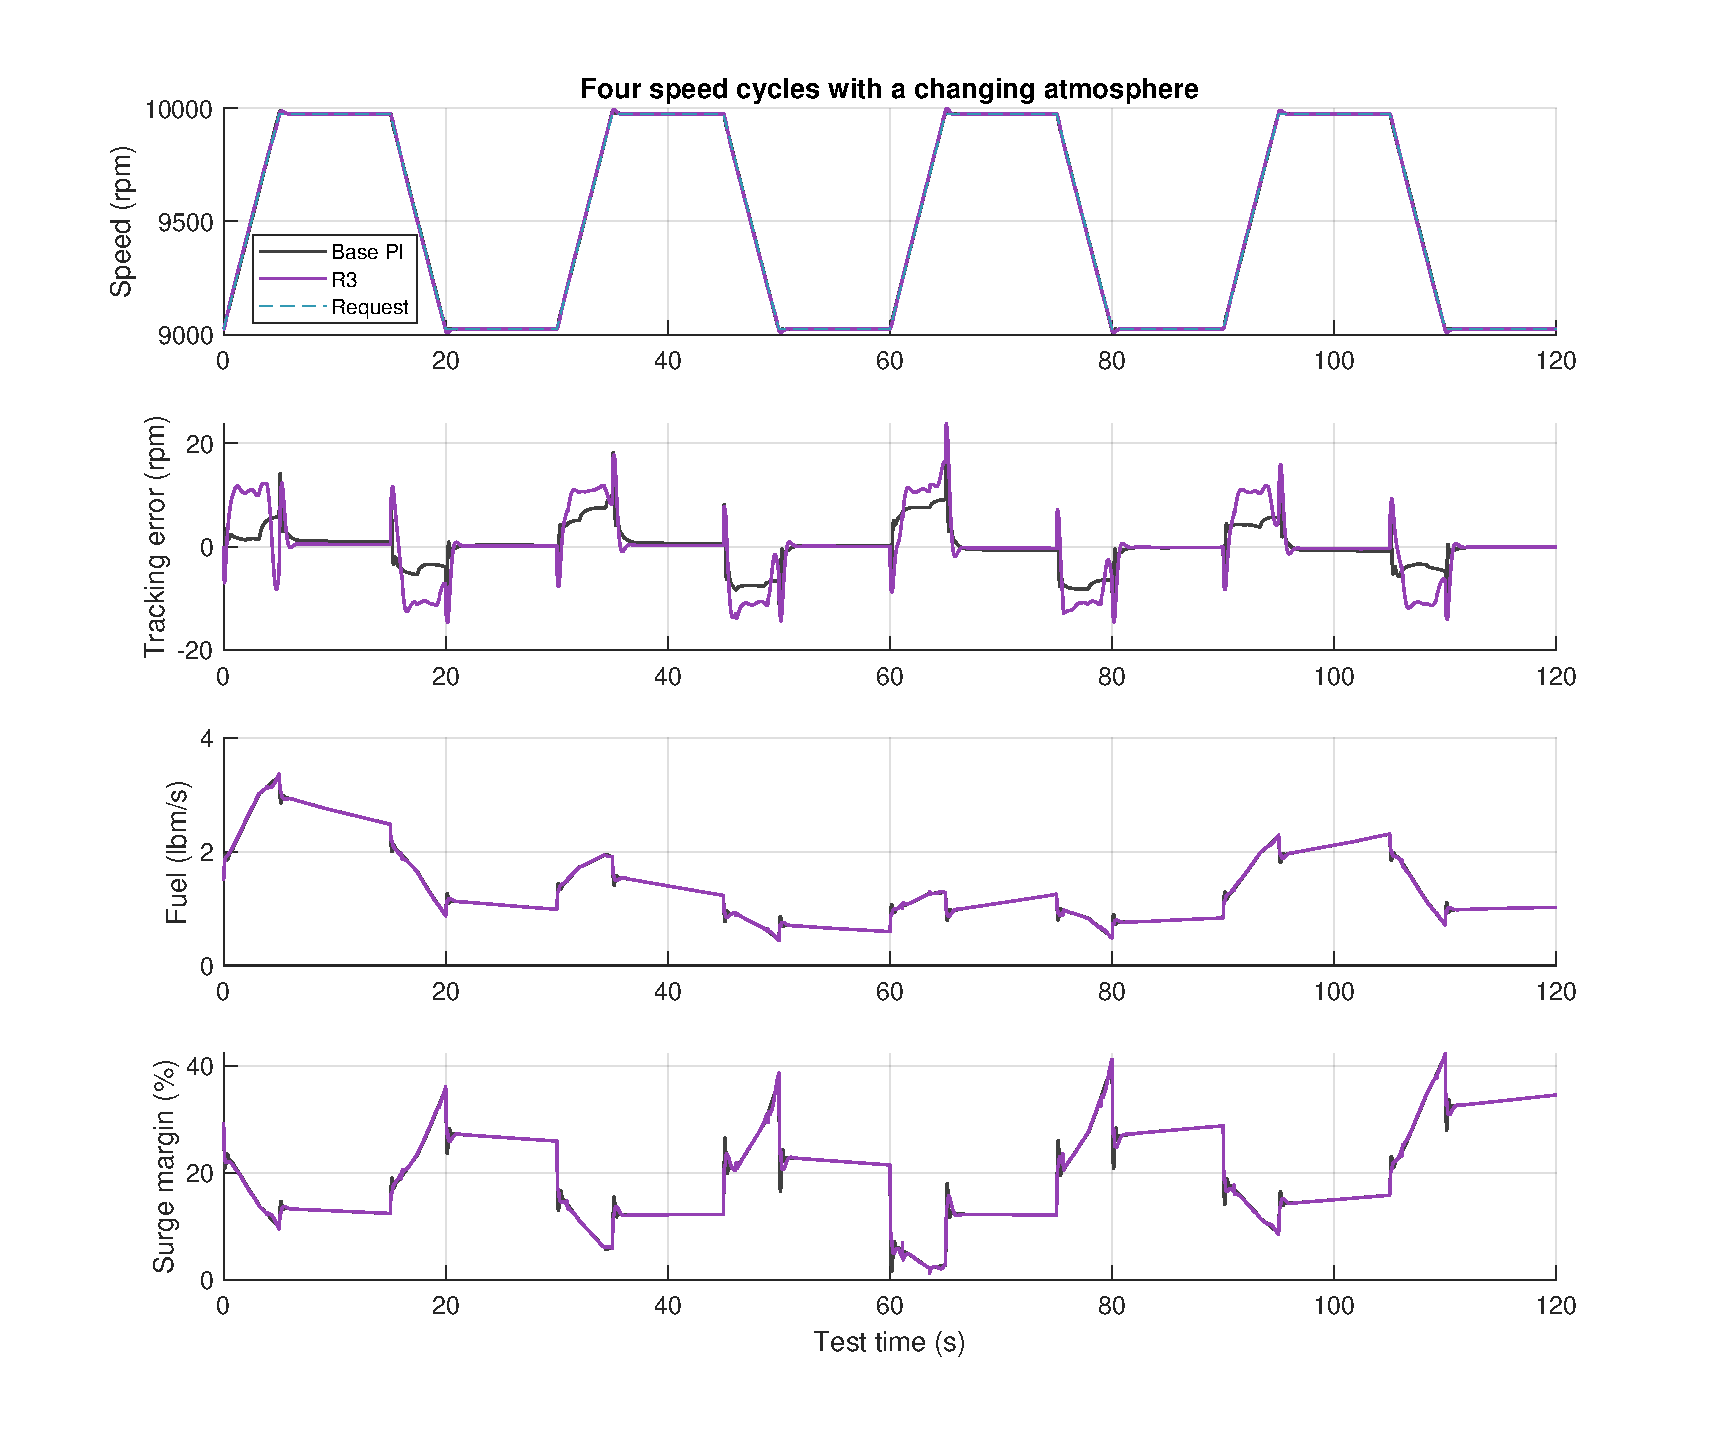
\includegraphics[width=\linewidth]{cycle_overview.pdf}\caption{Full 120 s test; the separate preparation interval is omitted.}\end{figure}
The request, actual speed, speed error, fuel and surge margin are recorded from the nonlinear plant simulation. A low hold RMSE alone does not establish satisfactory ramp tracking; both are retained in the table.
\clearpage
\section{Ambient evolution and fallback}
\begin{figure}[H]\centering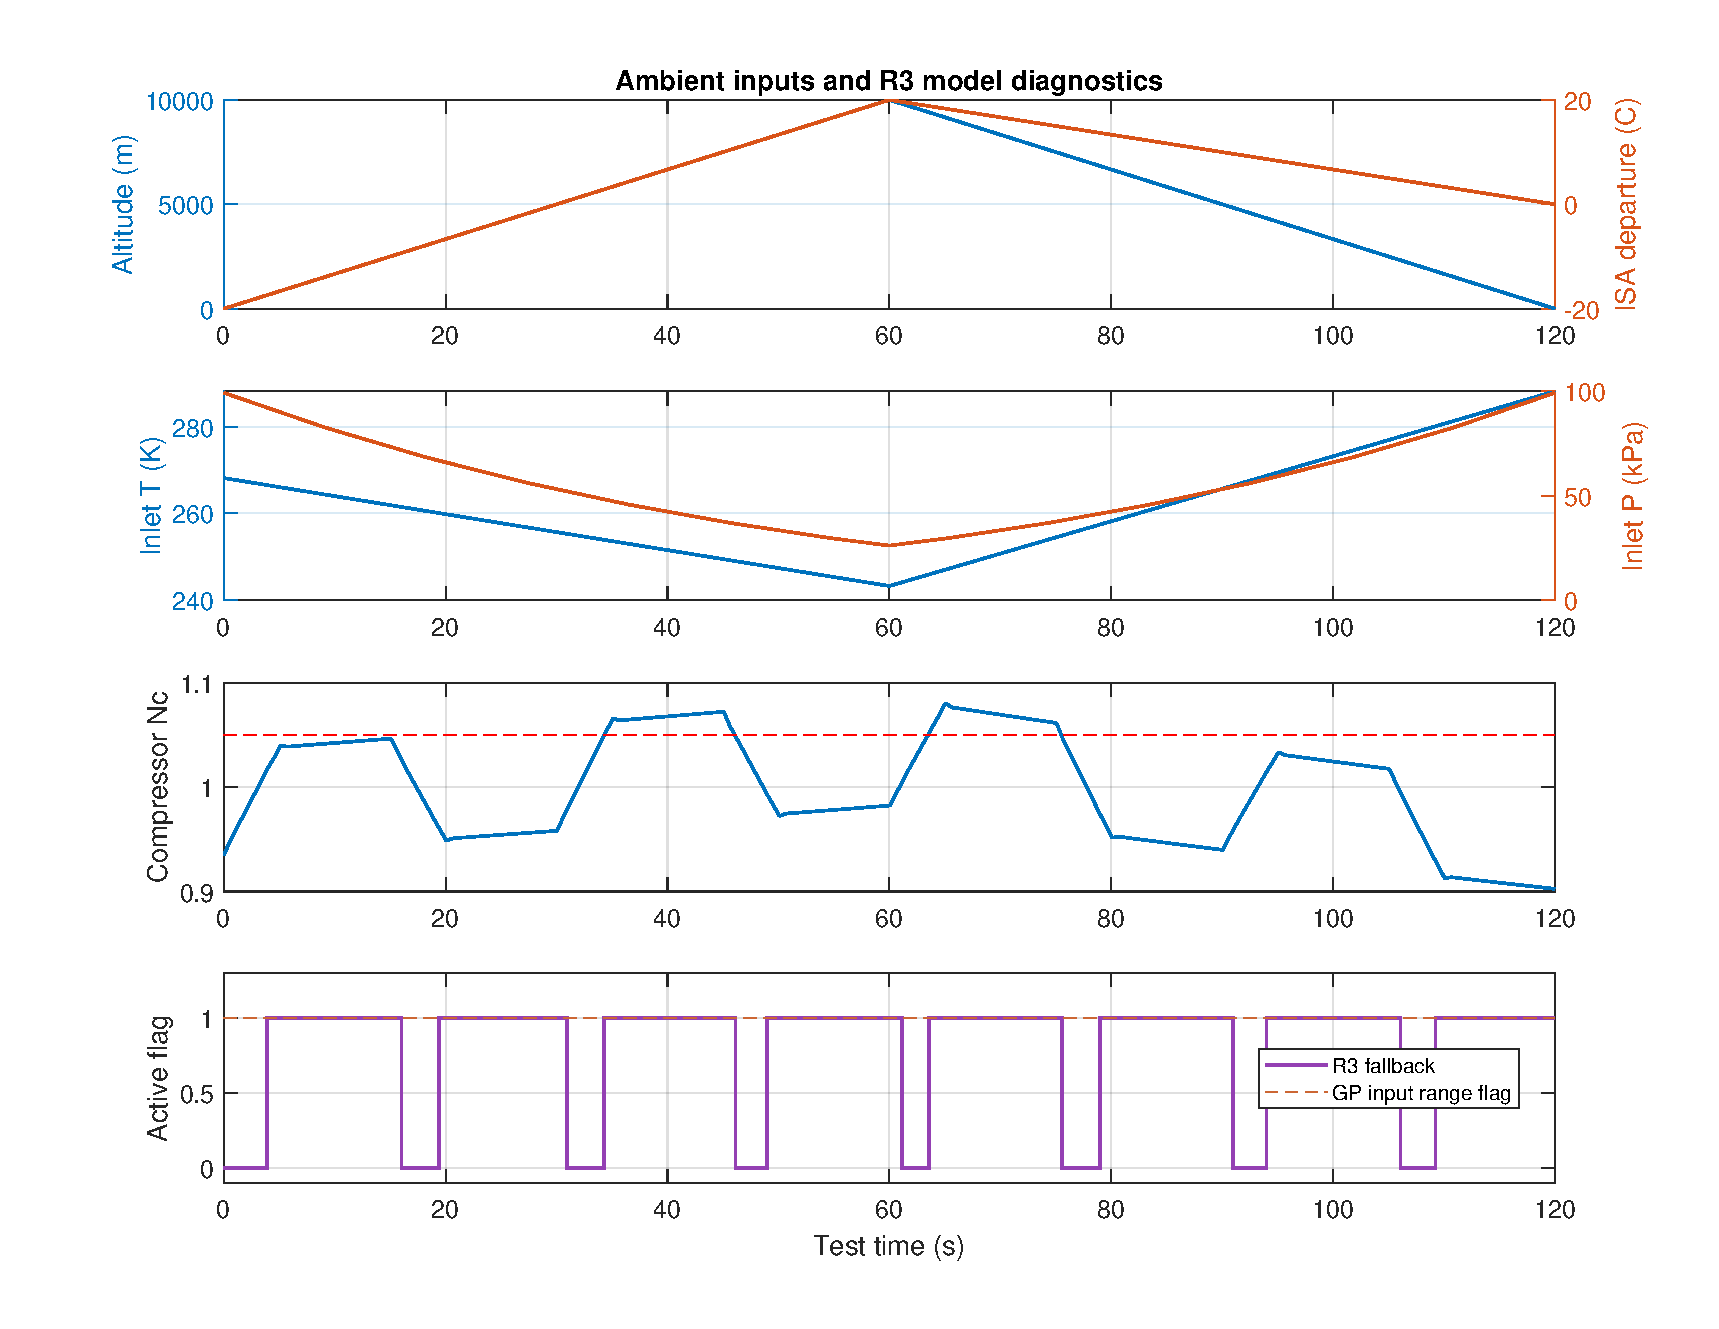
\includegraphics[width=\linewidth]{cycle_environment.pdf}\caption{Commanded environment, simulated inlet conditions, compressor map coordinate and R3 diagnostic flags.}\end{figure}
The fallback and training-range flags are distinct. A GP input-range flag tests the rectangular bounds of the training data, not posterior confidence or joint-density coverage. R3's fallback is driven by its existing slope/error/map guards. A controller can therefore query outside a training input range without immediately invoking fallback. Corrected-speed map overruns remain a limitation of the supplied engine simulation.
\clearpage
\section{Zoomed response: first cycle}
\begin{figure}[H]\centering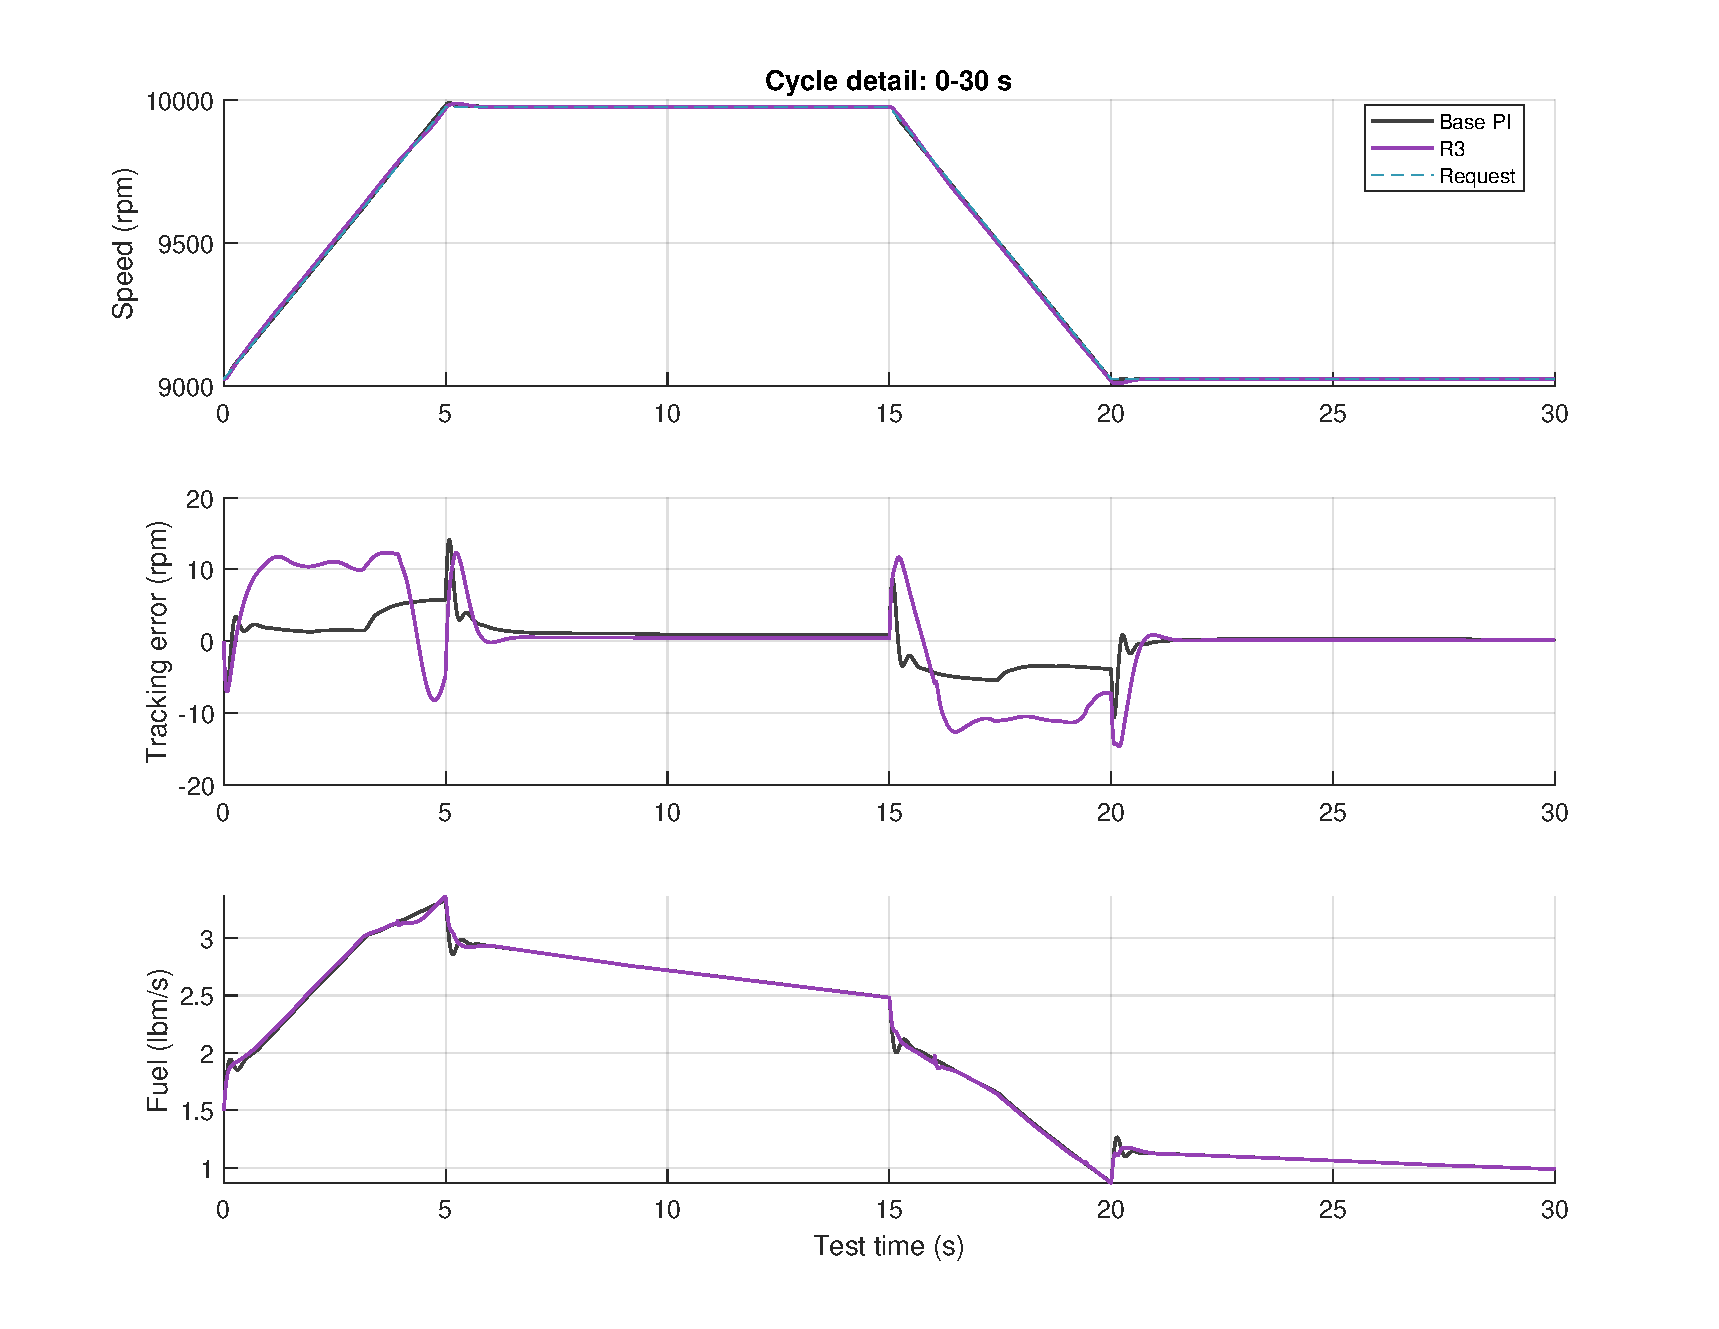
\includegraphics[width=\linewidth]{cycle_zoom_1.pdf}\caption{First acceleration, high hold, deceleration and low hold while the environment climbs away from sea level.}\end{figure}
\clearpage
\section{Zoomed response: ambient turning point}
\begin{figure}[H]\centering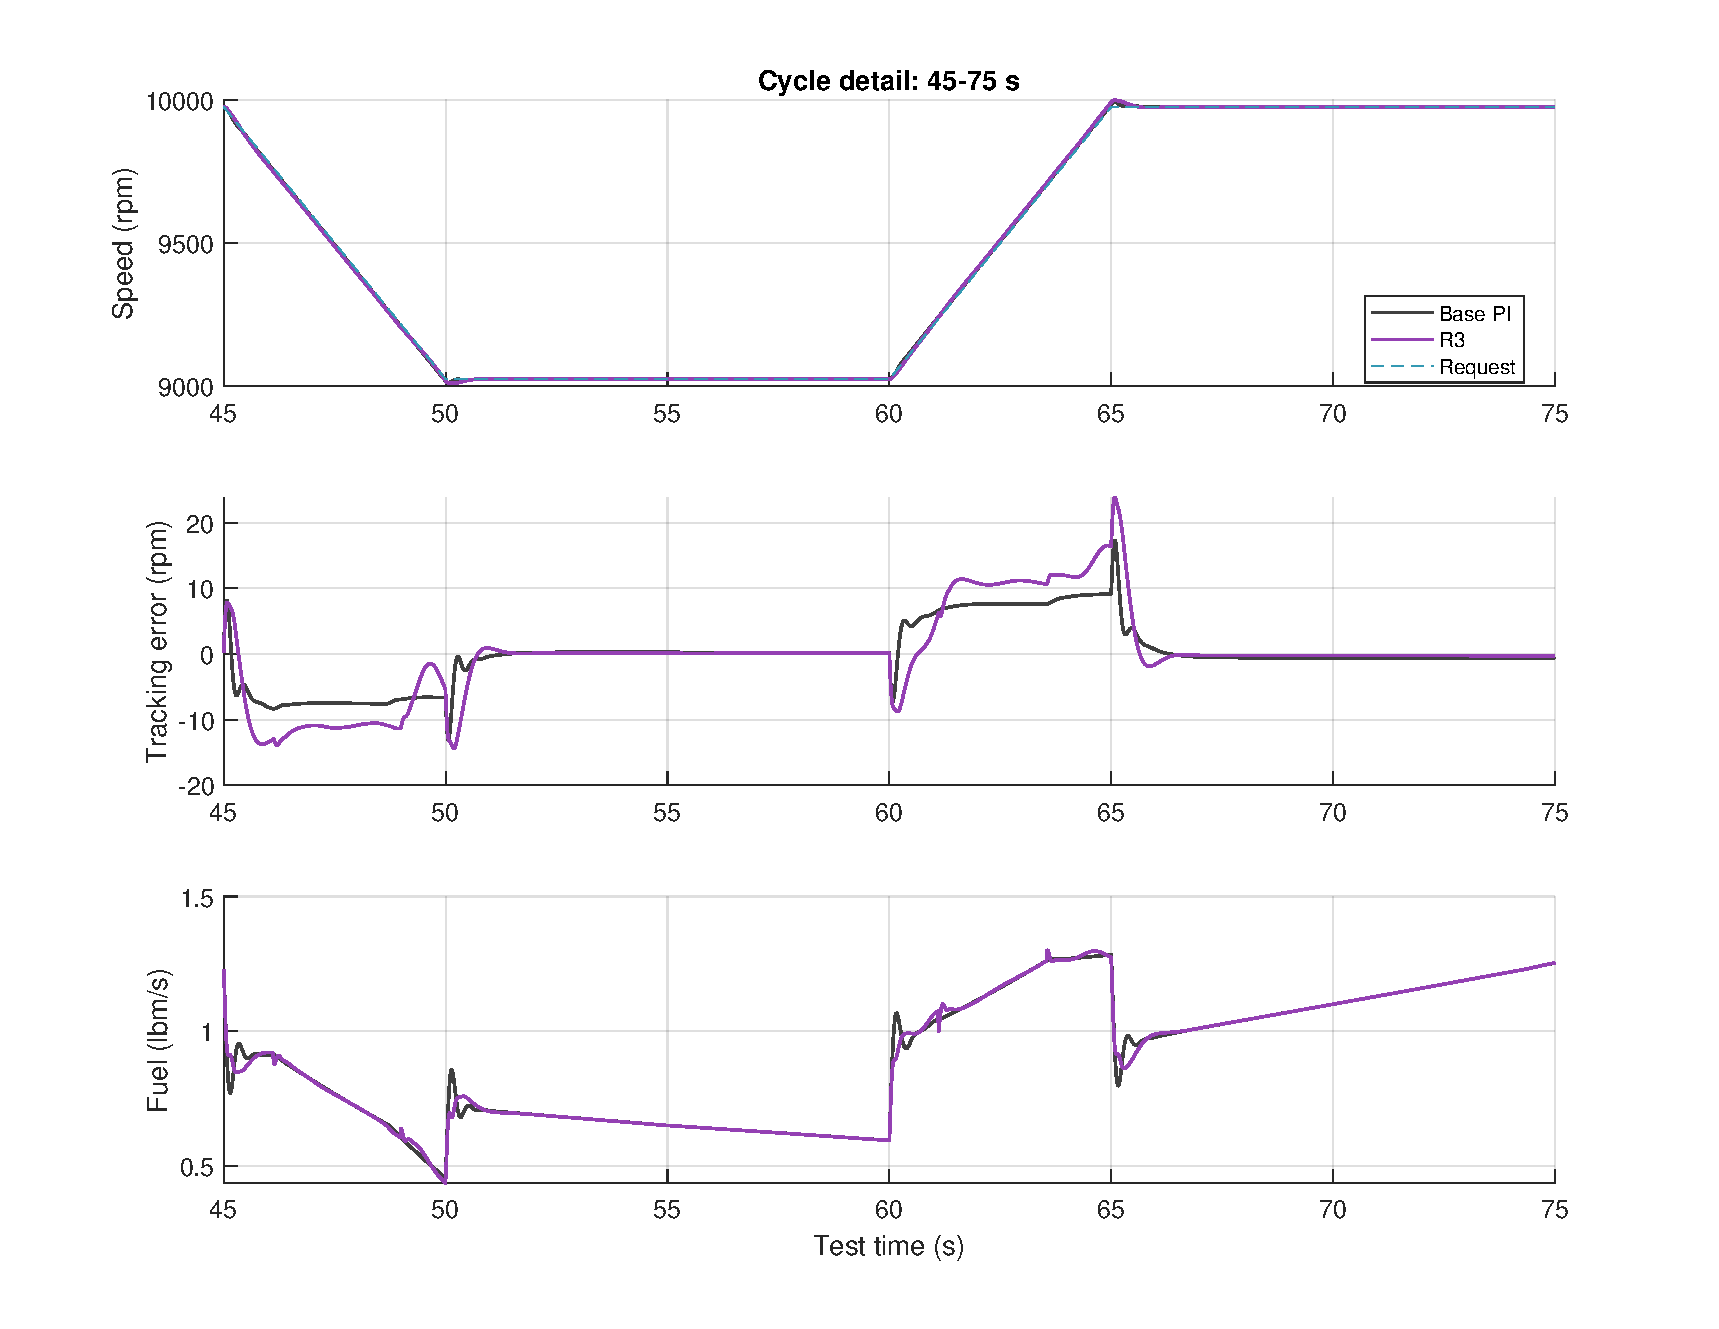
\includegraphics[width=\linewidth]{cycle_zoom_2.pdf}\caption{The 45--75 s window spans the 10000 m/ISA+20 turning point.}\end{figure}
The ambient direction reverses at 60 s, at the beginning of the third acceleration ramp. This window also includes the preceding deceleration and low-speed hold.
\clearpage
\section{All ramp and hold segments}
\begin{table}[H]\centering\small\begin{tabular}{llrrrr}\toprule
Time (s) & Phase & RMSE base & RMSE R3 & TV base & TV R3\\\midrule
0--5 & acceleration & 3.42 & 9.654 & 0.1778 & 0.08742\\
5--15 & high hold & 2.118 & 2.253 & 0.2662 & 0.02286\\
15--20 & deceleration & 4.186 & 9.927 & 0.2302 & 0.1643\\
20--30 & low hold & 1.119 & 2.621 & 0.6487 & 0.4146\\
30--35 & acceleration & 6.529 & 9.803 & 0.3034 & 0.1416\\
35--45 & high hold & 2.542 & 3.172 & 0.3561 & 0.1071\\
45--50 & deceleration & 7.169 & 10.14 & 0.4016 & 0.2969\\
50--60 & low hold & 1.455 & 2.56 & 0.6146 & 0.3585\\
60--65 & acceleration & 7.452 & 10.56 & 0.2662 & 0.3393\\
65--75 & high hold & 2.241 & 3.934 & 0.9443 & 0.7233\\
75--80 & deceleration & 7.294 & 9.957 & 0.4101 & 0.3767\\
80--90 & low hold & 1.433 & 2.6 & 0.3739 & 0.1172\\
90--95 & acceleration & 4.605 & 9.166 & 0.2351 & 0.09108\\
95--105 & high hold & 1.847 & 2.861 & 0.9073 & 0.7251\\
105--110 & deceleration & 4.14 & 9.318 & 0.2655 & 0.1655\\
110--120 & low hold & 1.162 & 2.531 & 0.354 & 0.1109\\
\bottomrule\end{tabular}\caption{Per-segment speed RMSE in rpm and excess fuel total variation in lbm/s. Ambient conditions continue changing during every hold.}\end{table}
\section{Reproduction and scope}
Open \path{GasTurbine_Cycle_BasePI.mdl} or \path{GasTurbine_Cycle_R3.mdl} in the existing T-MATS workspace. Their preload callback is \path{tmats_r3_cycle_setup.m}. The original controller models are preserved. Run \path{run_tmats_r3_cycle.m} to regenerate both trajectories and \path{report_tmats_r3_cycle.m} for plots. Native MAT and CSV traces, segment tables and configuration are saved under \path{results/r3_ambient_cycle_20260915}.

Full-run acceptance requires finite valid plant signals, converged flow residuals, positive fuel and surge margin, fewer than 200 solver iterations, a settled pre-test speed and the complete 180 s simulation. Map coverage is reported independently. These results are a frozen-controller transfer test for the stated speed limits, ambient route and deterministic sensor/plant assumptions; they do not replace testing with actuator dynamics or measurement noise.
\end{document}
